\subsection{Further experimental results}\label{app:more}

\paragraph{Edge cases.} Table~\ref{tab:edge} varies the minimum class size $m$ in three federations. The default $m=4$ is best or close to best. A larger $m$ discards classes and hence evidence, and the effect is strongest with small clients ($m=16$: ARI $0.28$, 30\% of the conflicting pairs merged), because clients then report few classes and share few discriminative ones. With extreme label skew ($\alpha=0.1$) and with small clients, ARI falls to $0.71$ and $0.66$ at the default, with 3.5\% and 9.3\% conflicting merges. Under extreme label skew these are the coverage failures anticipated in Remark~\ref{rem:scope}(d); with small clients the main cause is the smaller separation at a reference model trained on less data, as in the sample-size study. The table averages the four scenarios, including the label-only one, which explains $K<4$ for the default federation. The reliability floor $r_{\min}$ has no measurable effect between $0$ and $0.2$: over the 144 combinations of scenario, federation, seed and $m$, changing $r_{\min}$ changes ARI by at most $0.017$.

\begin{table}[!htbp]
\centering
\caption{Edge cases: minimum class size $m$ in three federations (Rotation, Label swap, \emph{Mixed + QS} and label-only scenarios, 3 seeds, $r_{\min}=0.02$).}\label{tab:edge}
\scriptsize
\setlength{\tabcolsep}{4pt}
\begin{tabular}{llcccc}
\toprule
Federation & $m$ & ARI & Conflict\% & $K$ & Low-evidence clients \\
\midrule
Default federation & 2 & 0.86 & 0.3 & 4.0 & 0.0 \\
 & 4 & 0.97 & 0.2 & 3.3 & 0.0 \\
 & 8 & 0.91 & 1.5 & 3.3 & 0.0 \\
 & 16 & 0.75 & 5.0 & 3.8 & 0.2 \\
\midrule
Extreme label skew ($\alpha=0.1$) & 2 & 0.72 & 3.1 & 3.5 & 0.0 \\
 & 4 & 0.71 & 3.5 & 3.7 & 0.0 \\
 & 8 & 0.64 & 6.0 & 3.8 & 0.0 \\
 & 16 & 0.61 & 8.7 & 3.7 & 0.0 \\
\midrule
Small clients (100 samples) & 2 & 0.66 & 6.1 & 3.9 & 0.0 \\
 & 4 & 0.66 & 9.3 & 3.2 & 0.0 \\
 & 8 & 0.55 & 15.0 & 3.2 & 0.0 \\
 & 16 & 0.28 & 30.1 & 2.9 & 2.4 \\
\bottomrule
\end{tabular}

\end{table}



\paragraph{Theory in practice.}
Figure~\ref{fig:theory} validates the theory on synthetic signatures with known ground truth ($p=512$, noise of effective rank 16). The disattenuated similarity is nearly unbiased for every half size $h$, whereas the raw cosine is biased by up to $-0.37$. Safety and maximality are reached with probability 1 once $h\ge64$ for all separations $\Delta\in[0.2,0.7]$, and exact recovery is reached under full class support. The required $h$ grows as $\Delta$ shrinks. Recovery of a minority group of 1, 2, 4 or 8 clients follows the same curve (Figure~\ref{fig:thminority} in Appendix~\ref{app:figs}), as Corollary~\ref{cor:sc} states.

\begin{figure}[!htbp]
\centering
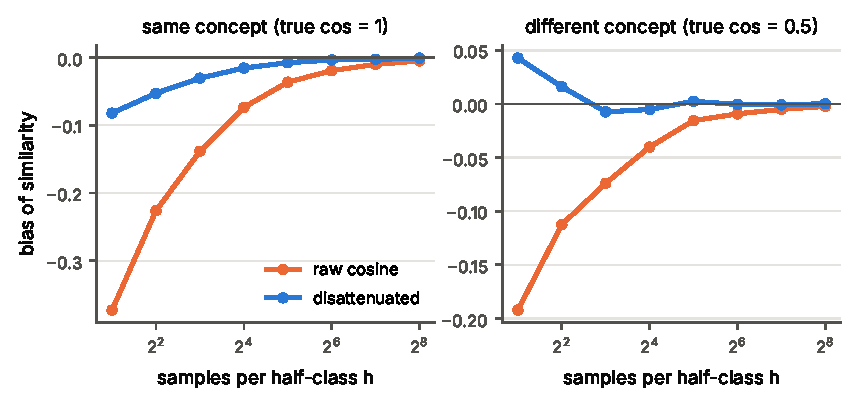
\includegraphics[width=0.49\linewidth]{theory_estimation.pdf}\hfill
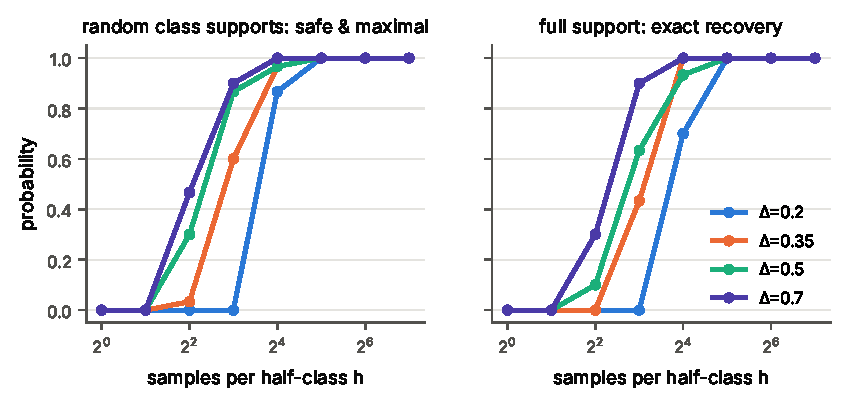
\includegraphics[width=0.49\linewidth]{theory_recovery.pdf}
\caption{Synthetic validation. Left: bias of the similarity estimate. Right: probability of the guarantees of Theorem~\ref{thm:rec}.}\label{fig:theory}
\end{figure}



\begin{tableorg}[!htbp]
\centering
\caption{Class-support disclosure under DP (rotation and label swap, 3 seeds). Plain: only the held classes are reported. Padded: noise vectors are sent for the other classes. Support acc.: accuracy of the server's guess ``class held iff $R_i^c>0$''; FPR: rate at which padded classes are guessed as held.}\label{tab:support}
\scriptsize
\setlength{\tabcolsep}{3pt}
\resizebox{\textwidth}{!}{%
\begin{tabular}{cccccccc}
\toprule
$\sigma$ & Samples/client & $\varepsilon$ & ARI plain & ARI padded & Support acc.\ plain (\%) & Support acc.\ padded (\%) & Support FPR padded (\%) \\
\midrule
0.5 & 400 & 10.00 & 0.43 & 0.26 & 91.3 & 77.2 & 38.1 \\
0.5 & 1500 & 10.00 & 0.75 & 0.45 & 92.2 & 83.9 & 35.3 \\
1 & 400 & 4.38 & 0.26 & 0.15 & 84.4 & 70.2 & 38.1 \\
1 & 1500 & 4.38 & 0.62 & 0.40 & 87.6 & 79.3 & 35.3 \\
2 & 400 & 1.99 & 0.08 & 0.10 & 77.0 & 62.9 & 38.1 \\
2 & 1500 & 1.99 & 0.48 & 0.32 & 81.7 & 73.3 & 35.3 \\
\bottomrule
\end{tabular}}

\end{tableorg}

\begin{table}[!htbp]
\centering
\caption{Concept drift after clustering (Fashion-MNIST, 3 seeds): detection rate of drifted clients, false-alarm rate on unchanged clients, and share of drifted clients reassigned to the cluster of their new group.}\label{tab:drift}
\scriptsize
\setlength{\tabcolsep}{4pt}
\begin{tabular}{llccc}
\toprule
Scenario & $q$ & Detection (\%) & False alarm (\%) & Reassigned correctly (\%) \\
\midrule
Rotation & 0.1 & 100.0 & 30.6 & 75.0 \\
Rotation & 0.2 & 100.0 & 59.4 & 54.2 \\
\midrule
Label swap & 0.1 & 100.0 & 45.4 & 66.7 \\
Label swap & 0.2 & 100.0 & 66.7 & 37.5 \\
\bottomrule
\end{tabular}

\end{table}

\begin{tableorg}[!htbp]
\centering
\caption{The complete pipeline with the default shrinkage $\lambda=0.5$ and with $\lambda=0.02$, for which the evidence condition of Theorem~\ref{thm:rec} can hold (Remark~\ref{rem:scope}(e)); all small-CNN scenarios (5 seeds; sweeps 3 seeds). $\Delta$: difference in mean accuracy (points). FMNIST: Fashion-MNIST; QS: quantity skew; part.: participation.}\label{tab:l02}
\scriptsize
\setlength{\tabcolsep}{3pt}
\resizebox{\textwidth}{!}{%
\begin{tabular}{lrccccccc}
\toprule
 & & \multicolumn{3}{c}{Accuracy (\%)} & \multicolumn{2}{c}{ARI} & \multicolumn{2}{c}{$K$} \\
\cmidrule(lr){3-5}\cmidrule(lr){6-7}\cmidrule(lr){8-9}
Scenario & $n$ & $\lambda=0.5$ & $\lambda=0.02$ & $\Delta$ & $\lambda=0.5$ & $\lambda=0.02$ & $\lambda=0.5$ & $\lambda=0.02$ \\
\midrule
FMNIST rotation & 5 & 89.1 & 89.1 & -0.0 & 0.92 & 0.92 & 4.4 & 4.4 \\
FMNIST label swap & 5 & 89.2 & 89.2 & -0.0 & 0.97 & 0.97 & 4.0 & 4.2 \\
FMNIST rotation + QS & 5 & 88.9 & 88.7 & -0.2 & 0.99 & 0.94 & 4.2 & 4.8 \\
FMNIST mixed + QS & 5 & 89.0 & 89.0 & +0.1 & 0.96 & 0.96 & 4.2 & 4.2 \\
FMNIST label skew only & 5 & 94.5 & 94.5 & -0.0 & 1.00 & 1.00 & 1.0 & 1.0 \\
FMNIST minority & 5 & 89.2 & 89.3 & +0.0 & 0.99 & 1.00 & 4.0 & 4.0 \\
MNIST rotation & 5 & 98.1 & 98.1 & -0.0 & 1.00 & 1.00 & 4.0 & 4.0 \\
MNIST label swap & 5 & 98.0 & 98.0 & +0.0 & 0.99 & 0.99 & 4.0 & 4.0 \\
KMNIST rotation & 5 & 86.9 & 87.1 & +0.2 & 0.96 & 0.98 & 4.2 & 4.2 \\
KMNIST label swap & 5 & 87.3 & 87.3 & +0.0 & 0.95 & 0.97 & 4.2 & 4.0 \\
EMNIST rotation & 5 & 84.2 & 83.8 & -0.3 & 0.98 & 0.95 & 4.4 & 4.6 \\
EMNIST label swap & 5 & 83.7 & 83.3 & -0.4 & 0.56 & 0.56 & 5.6 & 6.2 \\
SVHN rotation & 5 & 69.3 & 69.3 & +0.0 & 0.00 & 0.00 & 1.0 & 1.0 \\
SVHN label swap & 5 & 73.3 & 73.3 & +0.0 & 0.00 & 0.00 & 1.0 & 1.0 \\
CIFAR-10 rotation & 5 & 63.5 & 63.6 & +0.1 & 0.01 & 0.02 & 1.4 & 1.4 \\
CIFAR-10 label swap & 5 & 65.3 & 65.2 & -0.0 & 0.28 & 0.27 & 2.4 & 2.4 \\
Rotation $15^\circ$ & 3 & 88.7 & 88.5 & -0.2 & 0.52 & 0.44 & 2.7 & 2.7 \\
Rotation $30^\circ$ & 3 & 88.8 & 89.1 & +0.2 & 0.93 & 0.98 & 4.0 & 4.0 \\
Rotation $45^\circ$ & 3 & 89.1 & 89.1 & +0.0 & 1.00 & 1.00 & 4.0 & 4.0 \\
2 label permutations & 3 & 89.5 & 89.5 & -0.0 & 1.00 & 1.00 & 2.0 & 2.0 \\
8 label permutations & 3 & 88.2 & 88.2 & +0.1 & 0.79 & 0.81 & 8.7 & 8.7 \\
Rotation, 30\% part. & 3 & 87.1 & 87.0 & -0.0 & 0.93 & 0.98 & 4.3 & 4.0 \\
Label swap, 30\% part. & 3 & 87.3 & 87.3 & -0.1 & 0.98 & 0.98 & 4.0 & 4.0 \\
Rotation, 200 clients & 3 & 86.5 & 86.5 & +0.0 & 0.88 & 0.89 & 4.7 & 4.7 \\
\bottomrule
\end{tabular}}

\end{tableorg}

\begin{tableorg}[!htbp]
\centering
\caption{Dependence on the reference model (3 seeds). The reference model is trained for 10 rounds on all clients, on a random half of them, or on all clients except those of group 0; all clients are then clustered at that model. ARI (in/out): ARI among the clients that did and did not train the reference model. Merge g0: conflict-merge rate of the pairs that involve group 0. FMNIST: Fashion-MNIST; QS: quantity skew.}\label{tab:refmodel}
\scriptsize
\setlength{\tabcolsep}{3pt}
\resizebox{\textwidth}{!}{%
\begin{tabular}{lcccccccc}
\toprule
 & All clients & \multicolumn{4}{c}{Random half} & \multicolumn{3}{c}{Without group 0} \\
\cmidrule(lr){2-2}\cmidrule(lr){3-6}\cmidrule(lr){7-9}
Scenario & ARI & ARI & ARI (in) & ARI (out) & $K$ & ARI & $K$ & Merge g0 (\%) \\
\midrule
FMNIST rotation & 0.93 & 0.98 & 1.00 & 0.94 & 4.00 & 0.98 & 4.00 & 1.1 \\
FMNIST label swap & 0.98 & 0.98 & 1.00 & 0.95 & 4.00 & 0.98 & 4.00 & 0.0 \\
FMNIST mixed + QS & 0.96 & 0.93 & 1.00 & 0.91 & 4.00 & 0.96 & 4.00 & 0.0 \\
FMNIST label skew only & 1.00 & 1.00 & 1.00 & 1.00 & 1.00 & -- & -- & -- \\
MNIST rotation & 1.00 & 1.00 & 1.00 & 1.00 & 4.00 & 1.00 & 4.00 & 0.0 \\
MNIST label swap & 1.00 & 1.00 & 1.00 & 1.00 & 4.00 & 1.00 & 4.00 & 0.0 \\
\bottomrule
\end{tabular}}

\end{tableorg}

\begin{tableorg}[!htbp]
\centering
\caption{Calibration of the certificate standard errors on synthetic signatures (200 draws per setting; median over the 12 settings of cluster size $M\in\{3,6,12\}$ and number of classes $C\in\{2,5,10,20\}$ for each case and half size $h$). SD/se: standard deviation of $s_{iM}$ over draws divided by the mean standard error. Bias/se: mean error in units of the mean standard error. Coverage: fraction of draws whose $\pm2\,\mathrm{se}$ interval contains the population value, before and after removing the mean bias.}\label{tab:certgrid}
\scriptsize
\resizebox{\textwidth}{!}{%
\begin{tabular}{lrcccc}
\toprule
Case & $h$ & SD/se, median [range] & Bias / se & Coverage (\%) & Debiased coverage (\%) \\
\midrule
Same concept & 10 & 0.94 [0.86, 1.08] & -2.52 & 30 & 89 \\
 & 20 & 0.92 [0.80, 1.06] & -2.51 & 32 & 88 \\
 & 50 & 0.94 [0.81, 1.09] & -2.53 & 29 & 88 \\
 & 200 & 0.92 [0.84, 1.03] & -2.58 & 29 & 89 \\
Different, $\Delta=0.1$ & 10 & 1.09 [1.00, 1.22] & +0.20 & 81 & 81 \\
 & 20 & 1.13 [0.98, 1.27] & +0.13 & 80 & 82 \\
 & 50 & 1.16 [1.03, 1.23] & +0.10 & 80 & 80 \\
 & 200 & 1.13 [1.06, 1.46] & +0.10 & 80 & 80 \\
Different, $\Delta=0.3$ & 10 & 1.13 [1.01, 1.43] & +0.31 & 78 & 80 \\
 & 20 & 1.18 [1.13, 1.30] & +0.25 & 78 & 80 \\
 & 50 & 1.16 [1.06, 1.20] & +0.17 & 81 & 80 \\
 & 200 & 1.17 [1.04, 1.26] & +0.13 & 79 & 79 \\
\bottomrule
\end{tabular}}

\end{tableorg}

\begin{table}[!htbp]
\centering
\caption{Malicious clients (Fashion-MNIST rotation and label swap, 3 seeds each): ARI and conflict-merge rate among the honest clients, and the fate of the malicious clients (mean counts: isolated in a singleton, flagged as low-evidence or anomalous, merged into an honest cluster, or grouped only with other malicious clients).}\label{tab:byz}
\scriptsize
\setlength{\tabcolsep}{4pt}
\begin{tabular}{llcccccc}
\toprule
Attack & $m$ & Honest ARI & Honest conflict\% & Isolated & Flagged & Merged & Other \\
\midrule
Random vectors & 1 & 0.95 & 0.4 & 0.33 & 0.67 & 0.00 & 0.00 \\
 & 2 & 0.95 & 0.4 & 0.00 & 2.00 & 0.00 & 0.00 \\
 & 4 & 0.96 & 0.1 & 0.00 & 4.00 & 0.00 & 0.00 \\
\midrule
Mimicry & 1 & 0.99 & 0.3 & 0.00 & 0.00 & 1.00 & 0.00 \\
 & 2 & 0.94 & 0.7 & 0.00 & 0.00 & 2.00 & 0.00 \\
 & 4 & 0.97 & 0.1 & 0.00 & 0.00 & 4.00 & 0.00 \\
\midrule
Sign flip & 1 & 0.95 & 0.4 & 1.00 & 0.00 & 0.00 & 0.00 \\
 & 2 & 0.95 & 0.4 & 1.67 & 0.00 & 0.00 & 0.33 \\
 & 4 & 0.96 & 0.1 & 1.67 & 0.00 & 0.00 & 2.33 \\
\bottomrule
\end{tabular}

\end{table}

\begin{tableorg}[!htbp]
\centering
\caption{Attempted remedies for the failures: full-layer signature and 30 warm-up rounds (3 seeds).}\label{tab:real_variants}
\scriptsize
\begin{tabular}{lccccc}
\toprule
Method & Acc & Concept & ARI & $K$ & Conflict\% \\
\midrule
\multicolumn{6}{l}{\textit{Office-Home (4 domains, 65 classes)}}\\
FedAvg & 68.7 & 58.1 & 0.00 & 1.0 & 100.0 \\
FeSEM & 68.1 & 54.6 & 0.05 & 4.0 & 37.7 \\
Oracle & 70.5 & 61.4 & 1.00 & 4.0 & 0.0 \\
DisCo-CFL (default) & 69.4 & 58.1 & 0.32 & 3.3 & 29.1 \\
DisCo-CFL, full-layer signature & 70.0 & 59.7 & 0.75 & 4.7 & 6.7 \\
DisCo-CFL, 30 warm-up rounds & 70.0 & 59.5 & 0.41 & 4.3 & 19.1 \\
\midrule
\multicolumn{6}{l}{\textit{CIFAR-100, rotations}}\\
FedAvg & 52.8 & 42.2 & 0.00 & 1.0 & 100.0 \\
FeSEM & 49.1 & 37.3 & -0.01 & 4.0 & 31.3 \\
Oracle & 51.7 & 41.3 & 1.00 & 4.0 & 0.0 \\
DisCo-CFL (default) & 50.8 & 39.7 & 0.06 & 3.0 & 56.3 \\
DisCo-CFL, full-layer signature & 50.8 & 39.9 & 0.32 & 3.7 & 27.8 \\
DisCo-CFL, 30 warm-up rounds & 52.2 & 41.4 & 0.01 & 2.3 & 71.0 \\
\bottomrule
\end{tabular}

\end{tableorg}

\begin{tableorg}[!htbp]
\centering
\caption{Ablation on CIFAR-100 with label-swap groups (3 seeds). Columns as in Table~\ref{tab:real_variants}.}\label{tab:real_ablation}
\scriptsize
\begin{tabular}{lccccc}
\toprule
Variant & Acc & Concept & ARI & $K$ & Conflict\% \\
\midrule
DisCo-CFL (full) & 57.7 & 46.5 & 0.93 & 4 & 1.5 \\
no attachment stage & 57.2 & 45.6 & 0.90 & 5 & 1.3 \\
\bottomrule
\end{tabular}

\end{tableorg}

\paragraph{Robustness sweeps.}
Table~\ref{tab:sweeps} varies one factor at a time on Fashion-MNIST: the strength of the concept shift, the number of groups, the fraction of participating clients and the number of clients. Baselines are given the true $K$ where they need it.

\begin{tableorg}[!htbp]
\centering
\caption{Robustness sweeps (Fashion-MNIST, 3 seeds; the $90^\circ$ row repeats the \emph{Rotation} scenario with 5 seeds). For DisCo-CFL: ARI, number of clusters, conflict-merge rate, accuracy and concept accuracy. For comparison: the best baseline on accuracy and on concept accuracy (in parentheses), and the Oracle's accuracy.}\label{tab:sweeps}
\scriptsize
\setlength{\tabcolsep}{3pt}
\resizebox{\textwidth}{!}{%
\begin{tabular}{llcccccccc}
\toprule
& & \multicolumn{5}{c}{DisCo-CFL} & & & \\
\cmidrule(lr){3-7}
Factor & Setting & ARI & $K$ & Conflict\% & Acc & Concept & Best baseline Acc & Best baseline Concept & Oracle Acc \\
\midrule
Strength & $\theta=15^\circ$ & 0.52 & 2.7 & 30.0 & 88.7 & 76.0 & 88.7 (PACFL) & 75.1 (PACFL) & 89.3 \\
Strength & $\theta=30^\circ$ & 0.93 & 4.0 & 1.7 & 88.8 & 76.3 & 88.3 (FedDAG-C) & 74.5 (PACFL) & 89.1 \\
Strength & $\theta=45^\circ$ & 1.00 & 4.0 & 0.0 & 89.1 & 77.0 & 89.3 (FedDAG-C) & 76.6 (FedDAG-C) & 89.2 \\
Strength & $\theta=90^\circ$ & 0.92 & 4.4 & 1.1 & 89.1 & 76.4 & 88.6 (FedDAG-C) & 74.3 (FL+HC) & 89.3 \\
Groups & $K=2$ & 1.00 & 2.0 & 0.0 & 89.5 & 78.2 & 89.3 (FL+HC) & 77.3 (FL+HC) & 89.5 \\
Groups & $K=4$ & 0.97 & 4.0 & 0.0 & 89.2 & 76.7 & 88.3 (FL+HC) & 72.6 (FL+HC) & 89.2 \\
Groups & $K=8$ & 0.79 & 8.7 & 1.7 & 88.2 & 70.7 & 87.2 (MTCFL) & 59.8 (MTCFL) & 88.6 \\
Participation 30\% & rotation & 0.93 & 4.3 & 0.8 & 87.1 & 72.3 & 86.9 (FedDAG-C) & 70.0 (FedDAG-C) & 87.2 \\
Participation 30\% & label swap & 0.98 & 4.0 & 0.0 & 87.3 & 73.1 & 85.7 (FedCCFA) & 66.4 (FL+HC) & 87.2 \\
Scale & $N=200$ & 0.88 & 4.7 & 2.9 & 86.5 & 73.1 & 85.2 (IFCA) & 70.6 (FedDAG-C) & 87.2 \\
\bottomrule
\end{tabular}}

\end{tableorg}

\paragraph{Strength of the shift.} With rotations of $0,\theta,2\theta,3\theta$ degrees, DisCo-CFL separates the groups perfectly at $\theta=45^\circ$ (ARI $1.00$) and almost perfectly at $30^\circ$ (ARI $0.93$). At $15^\circ$ neighbouring concepts are so close that their class-conditional gradients agree above the threshold: the estimated separation is $\hat\Delta=0.06$, below $1-\tau=0.1$ (Table~\ref{tab:diag}), and DisCo-CFL merges them (ARI $0.52$, $K=2.7$). This is what the separation assumption predicts: the method groups what it cannot tell apart, and the diagnostic shows it. It costs little, because nearby concepts can share a model: accuracy is 88.7\% against 89.3\% for the Oracle, equal to the best baseline (PACFL, given $K$). For $\theta\ge30^\circ$ DisCo-CFL is within $0.3$ points of the Oracle; at $45^\circ$ FedDAG-C is $0.2$ points more accurate.

\paragraph{Number of groups.} With $K=2$, $4$ and $8$ label-permutation groups, DisCo-CFL finds the number of groups without being told (2.0, 4.0 and 8.7 clusters). With $K=8$, recovery is incomplete (ARI $0.79$, 1.7\% of the conflicting pairs merged): with Dirichlet label skew, many clients hold few of the classes that distinguish two of the eight permutations, so coverage is weaker. Accuracy is within $0.4$ points of the Oracle for all $K$, and $0.2$--$1.0$ points above the best baseline; concept accuracy is $0.9$--$10.9$ points above the best baseline.

\paragraph{Partial participation.} When only 30\% of the clients take part in each round, the warm-up model is noisier. DisCo-CFL still recovers the groups (ARI $0.93$ and $0.98$) and matches the Oracle within $0.1$ points, $0.2$--$1.6$ points above the best baseline in accuracy and $2.3$--$6.7$ points in concept accuracy.

\paragraph{Number of clients.} With 200 clients of 200 samples each, DisCo-CFL reaches ARI $0.88$ with 2.9\% of the conflicting pairs merged. Accuracy is 86.5\% against 87.2\% for the Oracle and 85.2\% for the best baseline (IFCA, given $K$); concept accuracy is $2.5$ points above the best baseline.

\begin{tableorg}[!htbp]
\centering
\caption{Failure rates per dataset (\%): fraction of runs with ARI below $0.5$ in the scenarios with more than one group. FMNIST: Fashion-MNIST, including the robustness sweeps; (R): pretrained ResNet-18. Runs per cell: 10 per dataset with two scenarios (5 seeds each), 5 for Office-Home and AG News, and 49 for Fashion-MNIST (five main scenarios with 5 seeds, eight sweeps with 3; 25 for DisCo-noAttach, which is not run on the sweeps). ``--'': not run (PACFL and FedDAG-C need image inputs).}\label{tab:failure_ds}
{\scriptsize
\resizebox{\textwidth}{!}{%
\begin{tabular}{l c c c c c c c c c c c}
\toprule
Method & FMNIST & MNIST & KMNIST & EMNIST & SVHN & CIFAR-10 & PACS & Office-Home & CIFAR-100 (R) & CIFAR-10 (R) & AG News \\
\midrule
DisCo & 2 & 0 & 0 & 30 & 100 & 100 & 0 & 100 & 50 & 50 & 0 \\
DisCo-noAttach & 0 & 0 & 0 & 40 & 100 & 100 & 0 & 100 & 50 & 50 & 0 \\
IFCA & 80 & 40 & 80 & 80 & 100 & 100 & 90 & 100 & 100 & 80 & 20 \\
FeSEM & 84 & 70 & 70 & 60 & 100 & 100 & 100 & 100 & 100 & 90 & 100 \\
MTCFL & 100 & 100 & 100 & 100 & 100 & 100 & 100 & 100 & 100 & 100 & 100 \\
FL+HC & 37 & 20 & 30 & 50 & 100 & 100 & 100 & 20 & 70 & 60 & 100 \\
PACFL & 71 & 90 & 100 & 70 & 100 & 100 & 90 & 100 & 90 & 100 & -- \\
StoCFL & 100 & 100 & 100 & 100 & 100 & 100 & 100 & 100 & 100 & 100 & 100 \\
StoCFL-W & 100 & 100 & 100 & 100 & 100 & 100 & 100 & 100 & 100 & 100 & 100 \\
FedCCFA & 100 & 100 & 100 & 100 & 100 & 100 & 100 & 100 & 100 & 100 & 60 \\
FedDAG-C & 57 & 60 & 50 & 50 & 100 & 100 & 100 & 100 & 100 & 100 & -- \\
\bottomrule
\end{tabular}}
}

\end{tableorg}
